% $Header: /cvsroot/latex-beamer/latex-beamer/solutions/conference-talks/conference-ornate-20min.en.tex,v 1.6 2004/10/07 20:53:08 tantau Exp $

\documentclass{beamer}

% This file is a solution template for:

% - Talk at a conference/colloquium.
% - Talk length is about 20min.
% - Style is ornate.

\mode<presentation>
{
  \usetheme{Boadilla}
  % or ...

  \setbeamercovered{transparent}
  % or whatever (possibly just delete it)
}

\title{Persistent Skip Lists}

\subtitle{For Efficient Point Set Queries}

\author{Simon Pratt}
% - Give the names in the same order as the appear in the paper.
% - Use the \inst{?} command only if the authors have different
%   affiliation.

\institute[Carleton University]
{
  Carleton University
}
% - Use the \inst command only if there are several affiliations.
% - Keep it simple, no one is interested in your street address.

\date{August 30th, 2011}
% - Either use conference name or its abbreviation.
% - Not really informative to the audience, more for people (including
%   yourself) who are reading the slides online

\subject{Computer Science}
% This is only inserted into the PDF information catalog. Can be left
% out. 

% If you have a file called "university-logo-filename.xxx", where xxx
% is a graphic format that can be processed by latex or pdflatex,
% resp., then you can add a logo as follows:

% \pgfdeclareimage[height=0.5cm]{university-logo}{university-logo-filename}
% \logo{\pgfuseimage{university-logo}}

% If you wish to uncover everything in a step-wise fashion, uncomment
% the following command: 

%\beamerdefaultoverlayspecification{<+->}

\begin{document}

\section{Title}
\begin{frame}
  \titlepage
\end{frame}

% Structuring a talk is a difficult task and the following structure
% may not be suitable. Here are some rules that apply for this
% solution: 

% - Exactly two or three sections (other than the summary).
% - At *most* three subsections per section.
% - Talk about 30s to 2min per frame. So there should be between about
%   15 and 30 frames, all told.

% - A conference audience is likely to know very little of what you
%   are going to talk about. So *simplify*!
% - In a 20min talk, getting the main ideas across is hard
%   enough. Leave out details, even if it means being less precise than
%   you think necessary.
% - If you omit details that are vital to the proof/implementation,
%   just say so once. Everybody will be happy with that.

\section{Motivation}

\subsection{Point Set Queries}

\begin{frame}
  \frametitle{Point Set Queries}

  \begin{itemize}
  \item
    Given a set of points in $\Re^2$
  \item
    Perform efficient 2 and 3 sided queries on the set of points
  \end{itemize}
\end{frame}

\begin{frame}
  \frametitle{Example Point Set Queries}
  % - A title should summarize the slide in an understandable fashion
  %   for anyone how does not follow everything on the slide itself.

  LeftMostNE

  \begin{itemize}
  \item
    Return the left most point bounded by $y_{min}$ and $x_{min}$
  \end{itemize}

    Enumerate3Sided

  \begin{itemize}
  \item
    Return all points bounded by $y_{min}$, $x_{min}$ and $x_{max}$
  \end{itemize}

\end{frame}

\subsection{Previous Work}

\begin{frame}
  \frametitle{In-Place Priority Search Trees}

  \begin{itemize}
  \item
    In-Place Data Structure which provides the same queries
  \item
    Binary tree
  \item
    Root node is highest y-coordinate
  \item
    Left and right subtrees are split along the median x-coordinate of
    the rest of the points
  \end{itemize}

\end{frame}

\begin{frame}
  \frametitle{Persistence}

  \begin{itemize}
  \item
    A new version of the data structure is saved upon each update
  \item
    Old versions of the data structure are queryable
  \item
    Some data structures work well for queries on a point set in $\Re$
  \item
    Can extend such a data structure to $\Re^2$ using persistence
  \end{itemize}

\end{frame}

\begin{frame}
  \frametitle{Skip List!}

  \begin{center}
    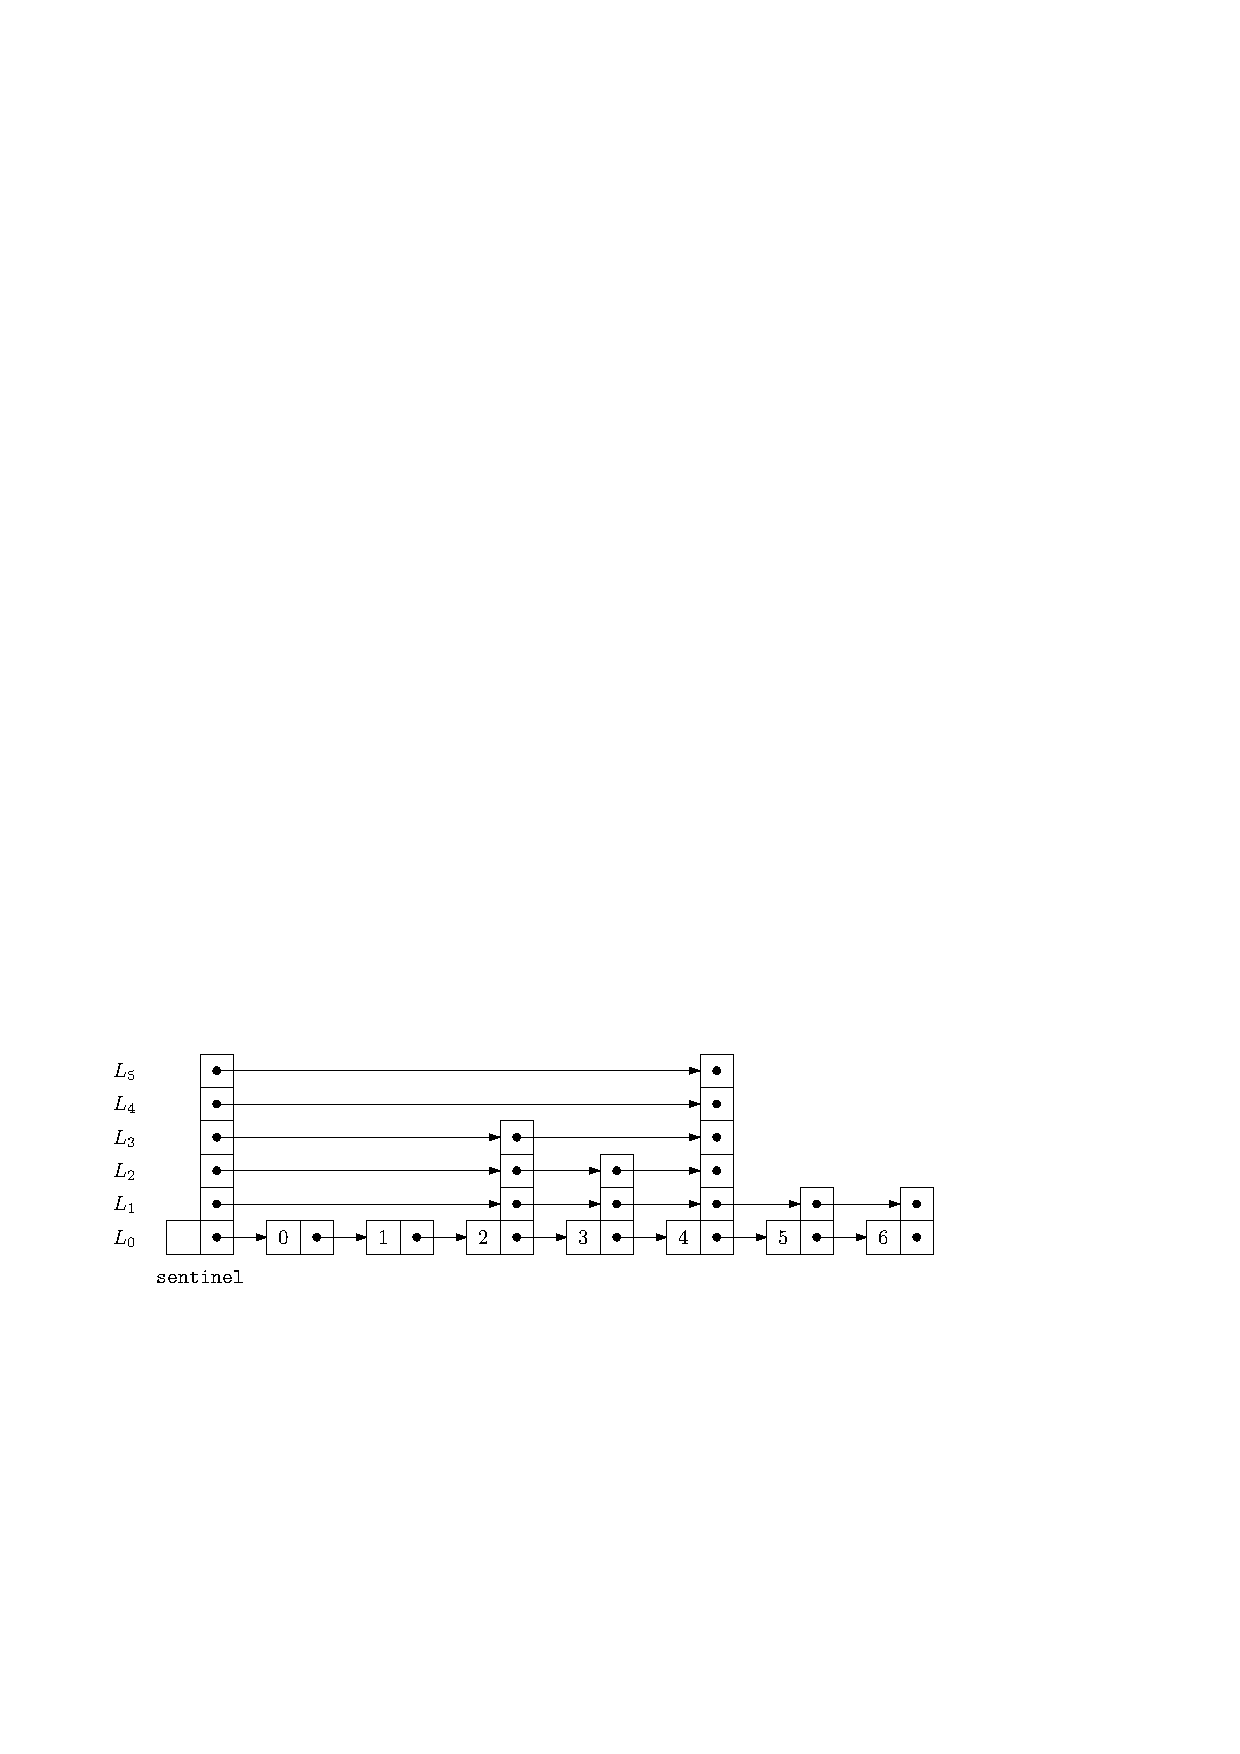
\includegraphics[width=300px]{figs/skiplist.pdf}
  \end{center}

\end{frame}

\section{Persistent Skip Lists}

\subsection{Solution}

\begin{frame}
  \frametitle{Persistent Skip List Design}

  \begin{itemize}
  \item
    Path Copying
  \item
    Fat Nodes
  \item
    Limited Path Copying with Fixed-Size Fat Nodes
  \end{itemize}

\end{frame}

\begin{frame}
  \frametitle{Performing Point Queries}

  \begin{itemize}
  \item
    An array A of points sorted by y-coordinate
  \item
    So the skiplist at a given timestamp corresponds to all of the points at or
    above the point at location timestamp in A
  \end{itemize}

\end{frame}

\begin{frame}
  \frametitle{Build Time}

  Given a randomly arranged array of unique points:
  \begin{itemize}
  \item
    O(logn) to sort points by y coordinate
  \item
    O(logn) to insert a single point into the skiplist
  \item
    O(nlogn) to perform n O(logn) insertions
  \end{itemize}

\end{frame}

\subsection{Algorithms}

\begin{frame}
  \frametitle{LeftMostNE}

  \begin{itemize}
  \item
    binary search on A to find lowest point higher than y bound
  \item
    skip list traversal to find left most point to the right of x bound
  \item
    Time complexity: O(logn)
  \end{itemize}

\end{frame}

\begin{frame}
  \frametitle{Enumerate3Sided}

  \begin{itemize}
  \item
    binary search on A to find lowest point higher than y bound
  \item
    skip list traversal to find left most point to the right of left x bound
  \item
    traverse lowest list linearly reporting all encountered points
    until finding the first point to the right of the right x bound
  \item
    Time complexity O(logn + k), where k is the number of points in the 
    query region
  \end{itemize}
\end{frame}

\subsection{Space Complexity}

\begin{frame}
  \frametitle{Space Complexity}

  \begin{itemize}
  \item
    Amortized space cost is the number of changes to the structure plus the
    change in potential
  \item
    Amortized space cost of an update is O(1)
  \item
    The sum of a sequence of amortized costs is O(n)
  \item
    This is an upper bound to the space complexity
  \end{itemize}  
\end{frame}

\section*{Summary}

\begin{frame}
  \frametitle<presentation>{Summary: Persistent Skip Lists}

  \begin{center}
    % Keep the summary *very short*.
    \begin{itemize}
    \item
      \alert{logarithmic} query time
    \item
      \alert{linear} space
    \item
      \alert{O(nlogn)} build time
    \end{itemize}
  \end{center}

\end{frame}

\begin{frame}
  \begin{center}
    {\bf Questions?}
  \end{center}
\end{frame}

% All of the following is optional and typically not needed. 
\appendix
\section*{Appendix}

\subsection*{For Further Reading}

\begin{frame}
  \frametitle<presentation>{Bibliography}

  \begin{thebibliography}{10}
    
  \beamertemplatebookbibitems
  % Start with overview books.

  \bibitem{Morin11}
    P. Morin
    \newblock {\em Open Data Structures}.
    \newblock Version 0.0 pre $\alpha$ : COMP2402 Fall 2011
    
  \beamertemplatearticlebibitems
  % Followed by interesting articles. Keep the list short. 

  \bibitem{DeMaheshwariNandySmid11}
    M. De, A. Maheshwari, S. C. Nandy, M. Smid.
    \newblock An In-Place Priority Search Tree
    \newblock
    {
      \em Proceedings of the 23rd Canadian Conference on Computational Geometry
    },
    331--336, August 2011.

  \bibitem{TarjanSarnak86}
    N. Sarnak and R. E. Tarjan.
    \newblock Planar Point Location Using Persistent Search Trees
    \newblock {\em Communications of the ACM},
    29(7):669--679, July 1986.

  \bibitem{Pugh90}
    W. Pugh.
    \newblock Skip lists: A probabilistic alternative to balanced trees.
    \newblock {\em Communications of the ACM},
    33(6):668--676, 1990.

  \end{thebibliography}
\end{frame}

\end{document}


